\documentclass{article}
\usepackage{listings}
\usepackage[utf8]{inputenc}
\usepackage{ amssymb }
\usepackage{amsfonts}
\usepackage{graphicx}

\title{Sistemas Distribuidos y Verificación \\ Tarea 3}
\author{Fabián Romero Jiménez}
\date{}
\begin{document}
\maketitle
\begin{enumerate}

\item[\bf{Problema 1}]  Recuerden el modelo visto en clase con el que resolvimos la tarea 
$\epsilon$-agreement para dos procesos. 
Alice y Bob proponen un valor y quieren quedar de acuerdo en un valor que no diste más $\epsilon$ de lo que el otro decidió. Después vimos que necesitaban comunicarse y que para $\epsilon$ más pequeñas se necesitaban más y más rondas de comunicación.
 Recuerden que usamos el modelo de memoria compartida de lectura/escritura por capas full information (por cada escritura leiamos un nuevo arreglo y escribimos todo lo que sabemos cada vez).\\
Ahora proponemos otros dos modelos de comunicación:\\
El modelo chismoso y el modelo discusión civil. El modelo chismoso dice que si de Alice
y Bob alguno de los 2 no escucho al otro entonces tienen otra ronda de comunicación.
 Si los dos se escuchan entonces ahi temina la comunicación.\\
Podriamos verlo como que se lanzan insultos e indirectas pero no de frente.\\
El modelo discusión civil dice que mientras Alice y Bob esten escuchando mutuamente la conversación sigue. En el momento que uno ya no escucha al otro ahi se termina.\\
Sea $M \ge 0$ el número de rondas máximo que se pueden comunicar Alice y Bob:
\newpage
\begin{enumerate}
\item Para los 2 modelos dados describe el complejo del protocolo $M$. Tienes que dar la tripleta $( I, P_m , \Xi_ m)$

\begin{enumerate}
\item Modelo chismoso:\\
En cada ronda de comunicación, se considerarán 2 tipos de aristas, aquellas donde hay comunicación bidireccional (y ya no participan en la proxima ronda) y aquellas donde no (que si participan en la próxima ronda), las que no tuvieron comunicación se trisectan como en el modelo visto en clase, pero la arista del medio resultante se marca como final y no participará en la próxima ronda de comunicación (punteadas en el dibujo) :\\
\begin{center}
  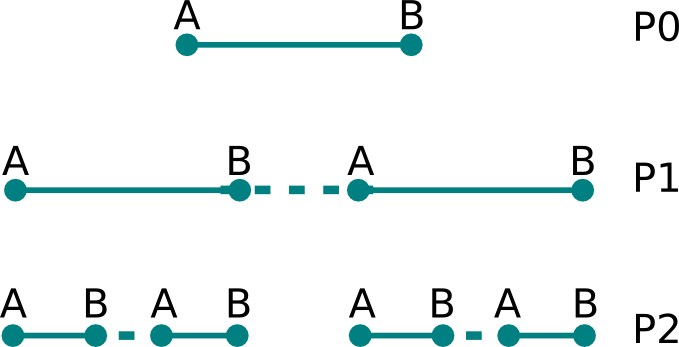
\includegraphics[width=200px]{t3f1.png}
\end{center}
Así, en la iteración $k$ habrá $2^k$ aristas que participan en la próxima iteración y $2^{k-1}$ aristas que no participan en la proxima iteración.
Así, el número de aristas está dado por:\\ $\#E(P_0)=1$, $\#E(P_i)=3*2^{i-1}$

\item Modelo discusión civil:\\
Sejemante al modelo anterior, $P_0$ y $P_1$ son idénticas, pero a partir de ahi, las que participan en la próxima ronda son las aristas punteadas, que en cada caso solo es una, así que de ahi en adelante, todos los niveles serán identicos.

\begin{center}
  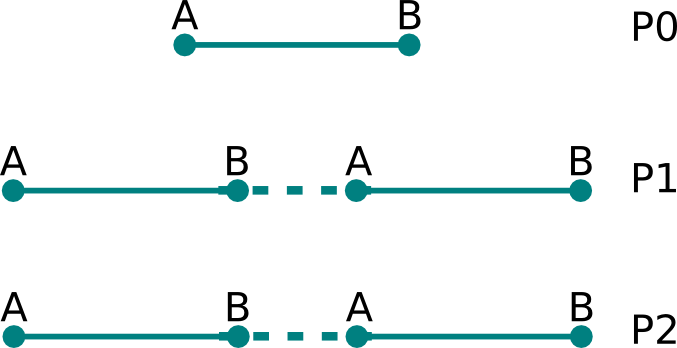
\includegraphics[width=200px]{t3f2.png}
\end{center}
\end{enumerate}

\item  Para los 2 modelos describe cuál es la tarea  $\epsilon$-agreement óptima para cada $M \ge 0$. Nos referimos a óptimo como que cada vista del protocolo va a un valor de decisión único.
En otras palabras, encontrar $\epsilon$ en función de M.
\end{enumerate}

\item[\bf{Respuesta}]
\begin{enumerate}
\item Modelo chismoso:\\
  Observe que si el protocolo termina en una linea punteada, se puede llegar a acuerdo, en caso de que no, se subdivide en $2^{M-1}$ aristas, por lo que se puede hacer un acuedo con $\epsilon = \frac{1}{2^{M-1}}$
\item Modelo discusión civil:\\
  En este caso, el protocolo pudo terminar en el primer paso, al no haber comunicación y sabemos que para ese caso, el mejor acuerdo es $\epsilon=\frac{1}{3}$ independientemente de la $M$
\end{enumerate}

\item[\bf{Problema 2}] Con el modelo visto en clase define la función de decisión de equidad de género $\delta$, que no distingue entre Alice y Bob. Es decir Alice y Bob pueden tener ya sea el valor 0 o 1 de entrada. También da la $\delta$ óptima para este caso. Aqui debes de tener cuidado de como etiquetas los vértices para que siempre se cumpla la $\epsilon$.

Etiquetemos basado en la cantidad de veces que ha visto cada digito como se muestra en la figura.

\begin{center}
  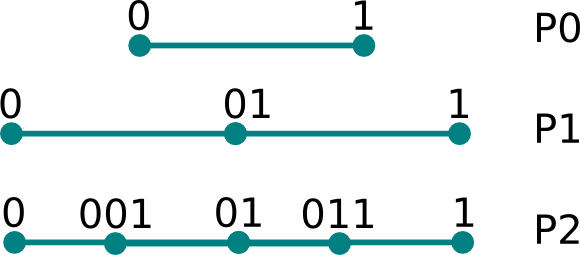
\includegraphics[width=200px]{t3f3.png}
\end{center}

así, cada ronda se duplica la cantidad de aristas, por lo que podemos dar una $\epsilon=\frac{1}{2^M}$

\item[\bf{Problema 3}] Ahora regresemos al modelo de memoria compartida y modifiquémoslo. Ahora supongamos que tenemos solo una memoria. Es decir ya no tenemos capas y sobrescribimos nuestra parte del arreglo cada ronda. También regresamos al caso en que Alice propone 0 y Bob 1.
\begin{itemize}
\item Describe el modelo (haz la gráfica) y ve como se ve la gráfica de vistas después de M rondas.

\begin{center}
  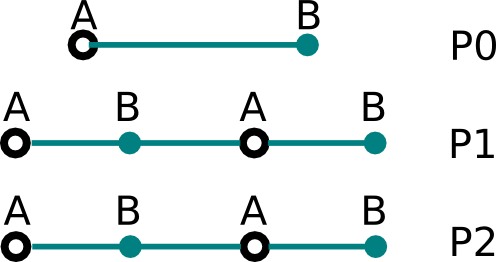
\includegraphics[width=200px]{t3f4.png}
\end{center}

En el inicio y primera ronda de comunicación, ambos modelos son claramente indistinguibles, a partir de ahi, ya no hay forma de acumular información, dejando solo tres casos posibles, identicos a la primera ronda, donde uno de los dos actua más rápido y escencialmente va solo (las orillas), donde uno sabe del otro, pero no viseversa, y donde ambos saben del otro.


\item ¿Cuál es la mejor $\epsilon$ que se puede resolver en la tarea del $\epsilon$ agreement en M rondas?\\

En este caso, como en la primera ronda de comunicación visto en clase, el mejor acuerdo es $\epsilon=\frac{1}{3}$
\end{itemize}





\end{enumerate}
\end{document}
